\documentclass{article}


% if you need to pass options to natbib, use, e.g.:
%     \PassOptionsToPackage{numbers, compress}{natbib}
% before loading neurips_2022


% ready for submission
\usepackage[final]{neurips_2022}


% to compile a preprint version, e.g., for submission to arXiv, add add the
% [preprint] option:
%     \usepackage[preprint]{neurips_2022}


% to compile a camera-ready version, add the [final] option, e.g.:
%     \usepackage[final]{neurips_2022}


% to avoid loading the natbib package, add option nonatbib:
%    \usepackage[nonatbib]{neurips_2022}


\usepackage[utf8]{inputenc} % allow utf-8 input
\usepackage[T1]{fontenc}    % use 8-bit T1 fonts
\usepackage{hyperref}       % hyperlinks
\usepackage{url}            % simple URL typesetting
\usepackage{booktabs}       % professional-quality tables
\usepackage{amsfonts}       % blackboard math symbols
\usepackage{nicefrac}       % compact symbols for 1/2, etc.
\usepackage{microtype}      % microtypography
\usepackage{xcolor}         % colors
\usepackage{graphicx}
\usepackage{float}



\title{Exploring the Sentiment of Steam Reviews with Naive Bayes and Support Vector Machine}


% The \author macro works with any number of authors. There are two commands
% used to separate the names and addresses of multiple authors: \And and \AND.
%
% Using \And between authors leaves it to LaTeX to determine where to break the
% lines. Using \AND forces a line break at that point. So, if LaTeX puts 3 of 4
% authors names on the first line, and the last on the second line, try using
% \AND instead of \And before the third author name.


\author{
  Puttisan Mukneam \\
  Pitzer College\\
  Claremont, CA 91786 \\
  \texttt{nmukneam@students.pitzer.edu}
}


\begin{document}


\maketitle


\begin{abstract}
In this project, we investigate the application of machine learning techniques for sentiment analysis on Steam game reviews. Two models were employed: a Naive Bayes classifier with varying Laplacian Smoothing parameters and a linear Support Vector Machine (SVM) with different regularization parameters (C). The models were implemented using Python 3.10 and the scikit-learn library. Additionally, the influence of stop word removal during the data cleaning process on model accuracy was examined. Performance metrics, including Mean Squared Error (MSE), Accuracy, and F1 score, were utilized to compare the models' effectiveness. The results revealed that the linear SVM model with C=100 achieved the highest accuracy in sentiment classification. Interestingly, while stop word removal enhanced the performance of the Naive Bayes classifier, it did not improve the accuracy of the SVM model. These findings highlight the potential of machine learning algorithms for sentiment analysis in Steam game reviews and offer valuable insights into the effects of different model parameters and data preprocessing techniques on classification accuracy.
\end{abstract}

\section{Steam}

Steam is a digital distribution platform developed by Valve Corporation, which provides video game developers with a platform to distribute their games and allows gamers to purchase and play those games. It also offers various additional features, such as game updates, friend lists, achievements, and cloud storage for game progress. As one of the largest digital distribution platforms for PC gaming, Steam has a massive user base and hosts thousands of games ranging from indie titles to AAA releases.

\subsection{Steam Reviews}

Steam allows users to write and submit reviews for the games they have played. These reviews are valuable sources of information for potential buyers, as they provide insights into the gameplay experience, performance, and overall satisfaction of the players. The dataset used in this project was obtained from Kaggle [1] and contains Steam game reviews submitted by users.

The dataset consists of several columns, including:

\begin{itemize}
\item \textbf{app\_id}: A unique Game ID on the Steam store.
\item \textbf{app\_name}: The name of the game being reviewed.
\item \textbf{review\_text}: The text of the review written by the user.
\item \textbf{review\_score}: Review sentiment, indicating whether the review recommends the game (1) or not (-1).
\item \textbf{review\_votes}: The count of whether the review was voted useful by another user or not.
\end{itemize}

\begin{figure}[H]
  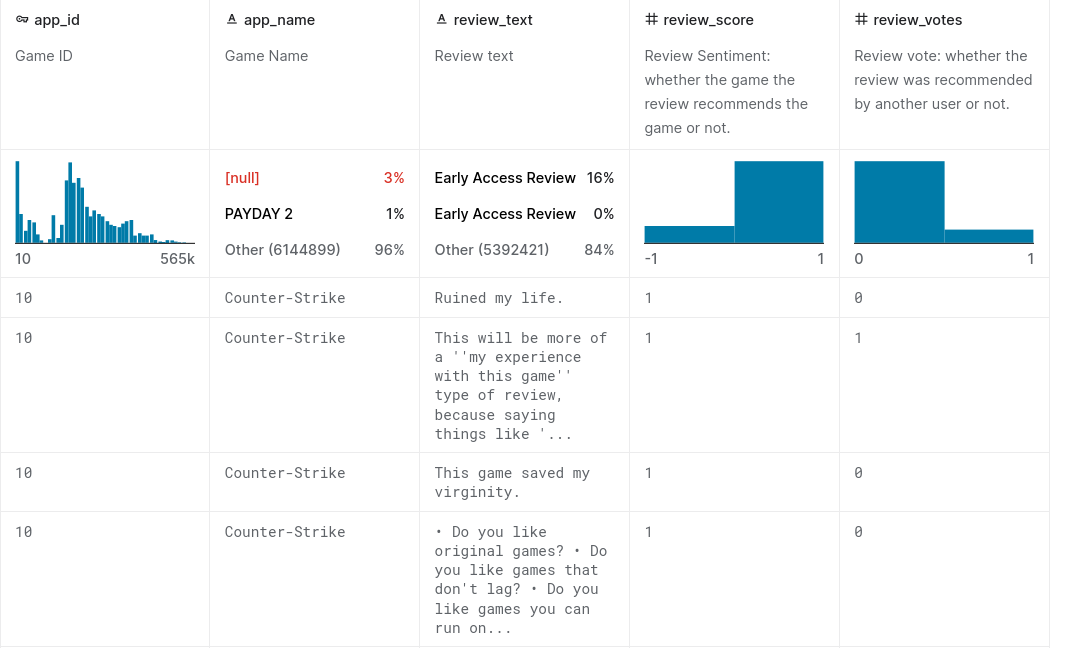
\includegraphics[width=12cm]{fig_1.png}
  \centering
  \caption{Steam Reviews [1]}
\end{figure}

In this project, we focus on the 'review\_text' and 'review\_score' columns to perform sentiment analysis. The 'review\_text' column provides the text data for analysis, while the 'review\_score' column serves as the sentiment label (positive if the game is recommended, negative otherwise).


\section{Data Processing}
There are various approaches to converting text data into numerical representations, such as Bag of Words, Word Embeddings, and Term Frequency-Inverse Document Frequency (TF-IDF). In this project, we use the TF-IDF method to represent the text data in the Steam reviews.
\subsection{TF-IDF}


TF-IDF is a widely used technique in information retrieval and text mining that captures the importance of words in a document relative to a collection of documents. It assigns a weight to each word based on its frequency in a document and its rarity across the entire document collection.

TF-IDF consists of two components:

\begin{itemize}
\item \textbf{Term Frequency (TF)}: It measures the frequency of a word in a document. A higher term frequency indicates the word is more important within the document. Mathematically, it can be expressed as:


   $$ TF(t, d) = \frac{f_{t, d}}{\sum_{t' \in d} f_{t', d}}$$


where $f_{t, d}$ is the frequency of term $t$ in document $d$ and the denominator represents the total frequency of all terms in the document.

\item \textbf{Inverse Document Frequency (IDF)}: It measures the rarity of a word across the entire collection of documents. Words that are more unique and rare receive higher IDF values. Mathematically, it can be expressed as:

    $$IDF(t, D) = \log \frac{N}{|\{d \in D : t \in d\}|}$$


where $N$ is the total number of documents in the collection $D$, and the denominator represents the number of documents containing the term $t$.

\end{itemize}

The TF-IDF weight for a word in a document is the product of its TF and IDF values:


$$TFIDF(t, d, D) = TF(t, d) \times IDF(t, D)$$


TF-IDF is chosen for this project due to its ability to balance the importance of words based on their frequency and rarity. It reduces the influence of common words, which appear in many documents but may not carry significant meaning for sentiment analysis. By representing the text data using TF-IDF, our machine learning models can better capture the relationships between the words in the reviews and their corresponding sentiment labels.

\subsection{Stopwords}

Stopwords are common words in a language that do not carry significant meaning and are often considered irrelevant or noise in text analysis tasks, such as sentiment analysis. Examples of stopwords in English include "a", "an", "the", "and", "in", "is", "of", "or", and "with", among others.

The primary reason for removing stopwords is to reduce the dimensionality of the text data and improve the efficiency of the analysis process. By eliminating these high-frequency, low-importance words, we can focus on the more meaningful and relevant words in the text, which are likely to have a stronger impact on the sentiment expressed in the review.

Additionally, removing stopwords can help improve the performance of certain machine learning models, such as the Naive Bayes classifier, by reducing the influence of common words on the model's predictions. However, it is essential to note that the impact of stopword removal on model performance may vary depending on the specific model and dataset used.

\section{Sentiment Analysis}

Sentiment analysis, also known as opinion mining, is a subfield of natural language processing (NLP) that focuses on extracting subjective information from text data. The primary goal of sentiment analysis is to determine the sentiment or emotional tone behind a series of words, which can be used to understand the attitudes, opinions, and emotions expressed by the author. Sentiment analysis is widely applied in various domains, including social media monitoring, product reviews, customer feedback analysis, and market research, among others.

There are various approaches to sentiment analysis, such as Lexicon-Based Methods, Machine Learning Methods, and Hybrid Methods. In this project, we will focus on Machine Learning Methods for sentiment analysis.

\subsection{Naive Bayes}

The Naive Bayes classifier is a probabilistic machine learning model based on Bayes' theorem, which is commonly used for text classification tasks such as sentiment analysis. It assumes that the features (words in our case) are conditionally independent given the class label, which simplifies the computation of probabilities.

Given a document $d$ and a class label $c$, Bayes' theorem can be expressed as:

\begin{equation}
P(c|d) = \frac{P(d|c)P(c)}{P(d)}
\end{equation}

The goal is to compute the probability $P(c|d)$ for each class and choose the class with the highest probability. Since the denominator $P(d)$ remains constant for all classes, we can ignore it and focus on the numerator:

\begin{equation}
P(d|c)P(c) = P(w_1, w_2, \dots, w_n|c)P(c)
\end{equation}

where $w_1, w_2, \dots, w_n$ are the words in the document.

Applying the conditional independence assumption, we can rewrite the probability as:

\begin{equation}
P(w_1, w_2, \dots, w_n|c)P(c) = P(c)\prod_{i=1}^{n} P(w_i|c)
\end{equation}

To classify a document, we choose the class $c^*$ with the highest probability:

\begin{equation}
c^* = \arg\max_c P(c)\prod_{i=1}^{n} P(w_i|c)
\end{equation}

\subsubsection{Laplacian Smoothing}

In practice, some words in the test data may not be present in the training data, leading to a zero probability for $P(w_i|c)$, which can cause issues in classification. To address this, Laplacian smoothing (also known as additive smoothing) is applied, which assigns a small non-zero probability to unseen words.

Given a word $w_i$ and a class $c$, the smoothed probability is calculated as:

\begin{equation}
P(w_i|c) = \frac{f_{w_i, c} + \alpha}{\sum_{w \in V} (f_{w, c} + \alpha)}
\end{equation}

where $f_{w_i, c}$ is the frequency of word $w_i$ in class $c$, $V$ is the vocabulary, and $\alpha$ is the smoothing parameter. A common choice for $\alpha$ is 1 (Laplace smoothing) or values between 0 and 1 (Lidstone smoothing).

\subsection{Linear Support Vector Machine (SVM)}

Support Vector Machines (SVM) are a class of supervised machine learning models used for classification and regression tasks. The main objective of an SVM is to find the optimal hyperplane that separates the data points of different classes with the maximum margin.

In the case of a linear SVM, the decision function is a linear combination of the input features:

\begin{equation}
f(x) = w^T x + b
\end{equation}

where $w$ is the weight vector, $x$ is the input feature vector, and $b$ is the bias term.

The goal is to minimize the following objective function:

\begin{equation}
\frac{1}{2} |w|^2 + C \sum_{i=1}^{n} \xi_i
\end{equation}

subject to the constraints:

\begin{equation}
y_i (w^T x_i + b) \geq 1 - \xi_i, \quad \xi_i \geq 0, \quad \forall i = 1, \dots, n
\end{equation}

where $n$ is the number of training examples, $y_i$ are the class labels, $\xi_i$ are the slack variables that allow some margin violations, and $C$ is a regularization parameter that controls the trade-off between maximizing the margin and minimizing the classification errors.


\section{Implementation}

To begin the implementation, we selected the first 1 million reviews out of over 6 million available reviews. This decision was made to avoid overloading the training machine and to strike a balance between dataset size and computational efficiency. We then divided the dataset into two parts: one for training (with local testing) and the other for testing using train\_test\_split function from scikit-learn library.

Next, we performed data cleaning by removing duplicate reviews, dropping rows containing NULL values, and removing special characters to ensure the quality and consistency of the dataset with the help of the NLTK package for providing stopwords in English.

The code is available in GitHub [2].

\subsection{Multinomial Naive Bayes}

We trained the Multinomial Naive Bayes classifier using various parameters for Laplacian smoothing. The MultinomialNB class from the scikit-learn library was utilized for this purpose. The results of the training process are presented below:

\begin{table}[h]
\centering
\begin{tabular}{llll}
\toprule
\textbf{Smoothing Parameter ($\alpha$)} & \textbf{Mean Squared Error} & \textbf{Accuracy} & \textbf{F-1 Score} \\
\midrule
0.001 & 0.53193 & 86.7018 & 0.92718 \\
0.01 & 0.53193 & 86.7018 & 0.92718 \\
0.1 & 0.53196 & 86.7011 & 0.92718 \\
0.5 & 0.53211 & 86.6972 & 0.92716 \\
1 & 0.53227 & 86.6933 & 0.92714 \\
2 & 0.53248 & 86.6879 & 0.92712 \\
3 & 0.53273 & 86.6818 & 0.92709 \\
\bottomrule
\end{tabular}
\caption{Multinomial Naive Bayes performance for different Laplacian smoothing parameters}
\label{table:naive_bayes_results}
\end{table}

\begin{table}[h]
\centering
\begin{tabular}{llll}
\toprule
\textbf{Smoothing Parameter ($\alpha$)} & \textbf{Mean Squared Error} & \textbf{Accuracy} & \textbf{F-1 Score} \\
\midrule
0.001 & 0.49789 & 87.5528 & 0.93152 \\
0.01 & 0.49789 & 87.5528 & 0.93152 \\
0.1 & 0.49789 & 87.5528 & 0.93152 \\
0.5 & 0.49814 & 87.5466 & 0.93149 \\
1 & 0.49826 & 87.5435 & 0.93148 \\
2 & 0.49854 & 87.5366 & 0.93144 \\
3 & 0.49881 & 87.5296 & 0.93141 \\
\bottomrule
\end{tabular}
\caption{Multinomial Naive Bayes performance for different Laplacian smoothing parameters (removed stopwords)}
\label{table:naive_bayes_results_removed_stopwords}
\end{table}



\subsection{Linear Support Vector Machine (SVM)}

We trained a Linear Support Vector Machine (SVM) classifier with various regularization parameter C values. The implementation was performed using the LinearSVC function from the scikit-learn library. The results of the training process are presented below:

\begin{table}[h]
\centering
\begin{tabular}{llll}
\toprule
\textbf{Regularization Parameter ($C$)} & \textbf{Mean Squared Error} & \textbf{Accuracy} & \textbf{F-1 Score} \\
\midrule
0.001 & 0.50156 & 87.461 & 0.93096 \\
0.01 & 0.40936 & 89.766 & 0.94211 \\
0.1 & 0.39620 & 90.095 & 0.94355 \\
1 & 0.39531 & 90.117 & 0.94362 \\
10 & 0.39534 & 90.117 & 0.94361 \\
100 & 0.39528 & 90.118 & 0.94362 \\
1000 & 0.39528 & 90.118 & 0.94362 \\
\bottomrule
\end{tabular}
\caption{Results for Linear SVM with various regularization parameter C values}
\label{table:svm_results}
\end{table}

\pagebreak

\begin{table}[h]
\centering
\begin{tabular}{llll}
\toprule
\textbf{Regularization Parameter ($C$)} & \textbf{Mean Squared Error} & \textbf{Accuracy} & \textbf{F-1 Score} \\
\midrule
0.001 & 0.48479 & 87.880 & 0.93323 \\
0.01 & 0.41010 & 89.747 & 0.94216 \\
0.1 & 0.40291 & 89.927 & 0.94287 \\
1 & 0.40238 & 89.940 & 0.94290 \\
10 & 0.40235 & 89.941 & 0.94290 \\
100 & 0.40235 & 89.941 & 0.94290 \\
1000 & 0.40238 & 89.940 & 0.94290 \\
\bottomrule
\end{tabular}
\caption{Results for Linear SVM with various regularization parameter C values (removed stopwords)}
\label{table:svm_results_removed_stopwords}
\end{table}

\subsection{Testing}
we decided to pick the Linear SVM with C=100 as the best model based on the previous results. We then used this model to test with our testing dataset. Here is the result:

\begin{table}[h]
\centering
\begin{tabular}{lll}
\toprule
\textbf{Mean Squared Error} & \textbf{Accuracy} & \textbf{F-1 Score} \\
\midrule
0.40112 & 89.97176 & 0.94282 \\
\bottomrule
\end{tabular}
\caption{Testing SVM with regularization parameter C = 100}
\label{table:svm_results}
\end{table}

\begin{table}[h]
\centering
\begin{tabular}{lll}
\toprule
\textbf{Mean Squared Error} & \textbf{Accuracy} & \textbf{F-1 Score} \\
\midrule
0.40473 & 89.88157 & 0.94251 \\
\bottomrule
\end{tabular}
\caption{Testing SVM with regularization parameter C = 100 (removed stopwords)}
\label{table:svm_results_removed_stopwords}
\end{table}


\section{Observations}
The lack of improvement in the SVM model after removing stop words may be attributed to several factors:
\begin{itemize}
    \item \textbf{High-dimensionality} SVMs are known for their ability to handle high-dimensional data effectively. Stop words, although they may not carry significant meaning, contribute to the high-dimensional feature space. The SVM model could have already captured the relationships between the remaining words and the sentiment labels, making the removal of stop words less impactful on the overall performance.
    \item \textbf{Noise reduction vs. information loss} While removing stop words can help reduce noise in the data, it may also lead to a loss of information. In certain contexts, stop words can contribute to understanding the sentiment of a text. By removing stop words, the SVM model might lose some of the subtle context-dependent information necessary for accurate sentiment analysis, counterbalancing the benefits of noise reduction.
    \item \textbf{Noise reduction vs. information loss} SVMs aim to find the optimal hyperplane that separates the classes with the largest margin. Removing stop words may not significantly alter the model's decision boundaries or the margin between the classes, resulting in minimal impact on the model's performance. This suggests that the presence or absence of stop words might not be a major factor influencing the complexity of the decision function.
    \item \textbf{Regularization parameter (C)} The SVM model's performance may also be influenced by the choice of the regularization parameter, C. A high value of C encourages the model to classify the training data more accurately, even at the risk of overfitting. In this case, the SVM model with C=100 may have already fit the data well, making the removal of stop words less beneficial for improving the model's performance. Adjusting the regularization parameter could potentially lead to different outcomes when comparing models with and without stop words.
\end{itemize}
Alternatively, though the SVM model demonstrated better overall performance, the Naive Bayes model also achieved impressive results. Furthermore, it has been shown that the Naive Bayes model can be as efficient as the Linear SVM model when enhanced using certain techniques, such as the removal of stop words. Both models can be considered suitable choices for sentiment analysis tasks, e.g., as we have demonstrated with this Steam Review dataset, depending on the specific requirements and the their configuration on a given task.

\section{References}
{
\small


[1] Sobkowicz, Antoni.  (2017). Steam Reviews Dataset\\ \url{https://www.kaggle.com/datasets/andrewmvd/steam-reviews}.


[2] Mukneam, Puttisan. sentiment\_steam. (2023).
\url{https://github.com/pmukneam/sentiment_steam}

[3] Konduru, Yaswanth Janardhan. (2021). Game Review Classifier. \url{https://yaswanth3277.github.io/Portfolio/gamereviewclassifier.html}

[4] Kumar, Satyam. (2018). IMDB movie review polarity using Naive Bayes Classifier.\\ \url{https://satyam-kumar.medium.com/imdb-movie-review-polarity-using-naive-bayes-classifier-9f92c13efa2d}

[5] Reddy, Vasista. (2018) Sentiment Analysis using SVM. \url{https://medium.com/@vasista/sentiment-analysis-using-svm-338d418e3ff1}

[6] Narayanan, Vivek., Aror, Ishan., Bhatia, Arjun. (2013). Fast and accurate sentiment classification using an enhanced Naive Bayes model. Indian Institute of Technology.

[7] Zuo, Zhen. (2018). Sentiment Analysis of Steam Review Datasets using Naive Bayes and Decision Tree Classifier. \url{http://hdl.handle.net/2142/100126}
\end{document}


